\documentclass[12pt,letterpaper]{article}

%\usepackage{cvpr}
%\documentclass[11pt,letterpaper]{article}
\setlength{\textheight}{8.875in}
\setlength{\textwidth}{6.875in}
\setlength{\columnsep}{0.3125in}
\setlength{\topmargin}{0in}
\setlength{\headheight}{0in}
\setlength{\headsep}{0in}
\setlength{\parindent}{1pc}
\setlength{\oddsidemargin}{-.304in}
\setlength{\evensidemargin}{-.304in}

\usepackage{times}
\usepackage{bbm}
\usepackage{epsfig}
\usepackage{graphicx}
\usepackage{amsmath}
\usepackage{amssymb}
\usepackage{amsthm}
\usepackage{mathrsfs}
\usepackage{caption}
\usepackage{subcaption}
\DeclareMathOperator*{\argmin}{\arg\!\min}
\newtheorem{lemma}{Lemma}
\newtheorem{proposition}{Proposition}
\newtheorem{theorem}{Theorem}
\newtheorem{coro}{Corollary}
\newtheorem{prop}{Property}
\newtheorem{definition}{Definition}

% If you comment hyperref and then uncomment it, you should delete
% egpaper.aux before re-running latex.  (Or just hit 'q' on the first latex
% run, let it finish, and you should be clear).



\def\texte#1{#1}

\begin{document}
\def\RR{\mathbb{R}}
\def\PP{\mathbb{P}}
\def\AA{\mathbb{A}}
\def\LL{\mathbb{L}}
\def\SS{\mathbb{S}}
\def\barr{\bar{\mathbb{R}}}
\def\mat#1{{\mathcal{#1}}}
\def\vect#1{\mbox{\boldmath $#1$}}
\def\PPi{\mbox{\boldmath$\Pi$}}
\def\squig{\rightsquigarrow}
%\def\vect#1{#1}
%\def\mat#1{#1}
\def\comment#1{{}}
%\def\qmatrix#1{\left[\begin{array}{l}#1\end{array}\right]}
\def\qmatrix#1{\left[\begin{matrix}#1\end{matrix}\right]}

\title{Kernel Square-Loss Examplar Machines}
\author{Jean Ponce}
%\date{}
\maketitle

\begin{abstract}
Zepeda and P\'erez show in~\cite{ZePe15} that the weight vectors
associated with examplar SVMs can be used as global features
representing images in tasks such as retrieval or classification. A
drawback is the cost of the procedure, which requires a (convex)
optimization process to be run for each positive image. This note
shows that a more efficient approach can be obtained using a square
loss instead of the hinge loss. Building on~\cite{BaJo05,FiSc01}, it
also shows that this approach is easily kernelized, and, assuming
low-rank kernels, that the corresponding computational cost is linear
in the number of negative examples for each positive example. The
presentation concludes with a brief discussion of the relationship
between the proposed approach with linear discriminant analysis and
its use in region matching in~\cite{ARS14}.
\end{abstract}


\section{Square-loss exemplar machines\label{sec:sqesvm}}
Given some loss function $l:[-1,+1]\times \RR\rightarrow \RR^+$, some
positive training example $x_0$ in $\RR^p$ and $n$ negative training
examples $x_i$ in $\RR^p$ ($i=1,\ldots,n$), training an exemplar
linear classifier consists in minimizing the error
\begin{equation} 
E(\omega,b)=\frac{1}{n}\sum_{i=1}^n l(-1,\omega^T x_i+b)+ \theta \ l(1,\omega^T x_0+b)+\frac{\lambda}{2} ||\omega||^2
\label{eq:general}
\end{equation} 
with respect to $\omega$ in $\RR^p$ and $b$ in $\RR$.

The traditional exemplar SVM uses the hinge loss for $l$. Let us use
instead the square loss. Equation~(\ref{eq:general}) becomes
\begin{equation}
E(\omega,b)=\frac{1}{2n}\sum_{i=1}^n (\omega^T x_i+b+1)^2+ \frac{\theta}{2}(\omega^T
x_0+b-1)^2+\frac{\lambda}{2} ||\omega||^2.
\label{eq:square}
\end{equation}

The interest of the square loss is that the minimization can be done
in closed form. Indeed, writing that $\partial E/\partial b=0$ at a
minimum yields
\begin{equation}
b=\dfrac{\theta-1}{\theta+1}-\dfrac{1}{\theta +1}(\theta x_0+\mu)^T \omega,
\end{equation}
where $\mu=\frac{1}{n}\sum_{i=1}^n x_i$ is the center of mass of the
negative samples $x_i$.

Substituting in Eq.~(\ref{eq:square}) now reduces our optimization problem
to the minimization with respect to $\omega$ of
\begin{equation}
\begin{array}{lcl}\hat{E}(\omega)&=&
\displaystyle\frac{1}{2n}\sum_{i=1}^n [\omega^T (x_i-\frac{1}{2}(x_0+\mu))+1]^2
+\frac{\theta}{2}[\omega^T (x_0-\frac{1}{2}(x_0+\mu))-1]^2+\frac{\lambda}{2}||\omega||^2\\
&=&
\displaystyle\min_{\omega\in\RR^p}
\frac{1}{2n}\sum_{i=1}^n [\omega^T (\sigma_i-\frac{1}{2}\delta) +1]^2
+\frac{\theta}{2}(\frac{1}{2}\omega^T\delta-1)^2+\frac{\lambda}{2}||\omega||^2,
\end{array}
\label{eq:weq}
\end{equation}
where $\delta=x_0-\mu$ and $\sigma_i=x_i-\mu$.

Finally, writing $\partial\hat{E}/\partial \omega=0$ at a minimum yields
\begin{equation}
\frac{1}{n}\sum_{i=1}^n [\omega^T(\sigma_i-\frac{1}{2}\delta)+1](\sigma_i-\frac{1}{2}\delta)
+\frac{1}{2}(\frac{1}{2}\omega\cdot\delta-1)\delta +\lambda \omega=0,
\end{equation}
or
\begin{equation}
[\frac{1}{n}\sum_{i=1}^n(\sigma_i-\frac{1}{2}\delta)(\sigma_i^T-\frac{1}{2}\delta^T)] \omega
+\frac{1}{n}\sum_{i=1}^n (\sigma_i-\frac{1}{2}\delta) +\frac{1}{2}\delta\frac{1}{2}\delta^T \omega -\frac{1}{2}\delta +\lambda \omega
=0.
\end{equation}

Using the fact that the variables $\sigma_i$ have zero
mean, we obtain
\begin{equation}
[\frac{1}{n}\sum_{i=1}^n\sigma_i\sigma_i^T +\frac{1}{2}\delta\delta^T +\lambda\text{Id}]
\omega=\delta,
\end{equation}
or, putting everything together and reverting to the original notation,
\begin{equation}
\left\{\begin{array}{l}
\displaystyle \omega=U^{-1} (x_0-\mu),\quad\text{where}\quad
U=\Sigma
+\frac{1}{2}(x_0-\mu)(x_0-\mu)^T +\lambda\text{Id},\\
\displaystyle b=-\frac{1}{2}(x_0+\mu)\cdot \omega,
\end{array}\right.
\label{eq:final}
\end{equation} 
where 
\begin{equation}
\Sigma=\frac{1}{n}\sum_{i=1}^n(x_i-\mu)(x_i-\mu)^T
=\frac{1}{n}\sum_{i=1}^n x_ix_i^T-\mu\mu^T=\frac{1}{n}X^TX-\mu\mu^T,
\label{eq:Sigmadef}
\end{equation}
is the covariance matrix of the negative samples $x_i$, and
$X$ denotes the $n\times p$ matrix with rows $x_i^T$ ($i=1,\ldots,n$).

The vector $\omega$ (or the vector $[\omega;b]$) of this {\em square-loss
examplar machine} can potentially be used as a new representation for
the corresponding positive feature $x_0$. Note that this gives
asymmetric roles to positive and negative examples.

A similar approach (with no regularizer) is advocated for region
matching in~\cite{ARS14}.  We will come back to this issue in the last
section of this presentation.



\section{Kernelized version}
Let us recall a few basic facts about kernel methods for supervised
classification. We consider a reproducing kernel Hilbert space (RKHS)
$H$ formed by real functions over some set
$X$, and denote by $k$ the corresponding reproducing kernel.  We
address the following learning problem over $H\times\RR$:
\begin{equation}
\min_{h\in H,b\in\RR}
\sum_{i=1}^n l[y_i,h(x_i)+b] + \frac{\lambda}{2}||h||^2,
\label{eq:kernel}
\end{equation}  
where the pairs $(x_i,y_i)$ ($i=1,\ldots,n$) in $X\times Y$ are
training samples, $Y=\RR$ (regression) or $Y=\{-1,1\}$
(classification), and $L: Y\times \RR\rightarrow\RR$ is some arbitrary
loss function. By definition of a reproducing kernel,
Eq.~(\ref{eq:kernel}) can be rewritten as
\begin{equation}
\min_{h\in H,b\in\RR}
\sum_{i=1}^n l[y_i,( \varphi(x_i)|h)+b] +
\frac{\lambda}{2}||h||^2,
\label{eq:kernelaff}
\end{equation} 
where $\varphi$ is the {\em feature map} over $X$ associated with the
kernel $k$ (which may not admit a known explicit form). We dub
problems with the general form of (\ref{eq:kernelaff}) {\em affine}
supervised learning problems since, given some fixed element $h$ of
$H$ and some scalar $b$, $(h|h')+b$ is an affine function of $h'$,
whose zero set defines an affine hyperplane of $H$ considered itself
as an affine space.


Let $K$ denote the kernel matrix with entries $k_{ij}=[\varphi(x_i)|
\varphi(x_j)]$ and rows $k_i^T$ ($i=1,\ldots,n$).  We assume from now
on that $L$ is convex and continuous. We have the following theorem.

\begin{theorem}\label{th:affinelearn}
Equation~(\ref{eq:kernelaff}) admits equivalent primal and dual versions. 

The primal problem is
\begin{equation}
\min_{\alpha\in\RR^n,b\in\RR} \sum_{i=1}^n l[y_i,k_i^T\alpha+b]
+\frac{\lambda}{2}\alpha^TK\alpha,
\label{eq:primal1}
\end{equation}
and any solution $(\alpha^\star,b^\star)$ to (\ref{eq:primal1})
provides
a solution $(h^\star,b^\star)$ to (\ref{eq:kernelaff}) with
$h^\star=\sum_{i=1}^n \alpha_i^\star\varphi(x_i)$.

Let $r$ denote the rank of the kernel matrix $K$, a 
{\em reduced} version of the primal problem is 
\begin{equation}
\min_{\beta\in\RR^r,b\in\RR}  \sum_{i=1}^n l[y_i,b_i^T\beta+b]
+\frac{\lambda}{2}||\beta||^2,
\label{eq:primal2}
\end{equation}
where $B$ is the $n\times r$ incomplete Cholesky decomposition of $K$ and $b_i^T$ denotes
its $i$th row,
and any solution $(\beta^\star,b^\star)$ to (\ref{eq:primal2})
provides
a solution $(h^\star,b^\star)$ to (\ref{eq:kernelaff}) with
$h^\star=\sum_{i=1}^n \alpha_i^\star\varphi(x_i)$, and
$\alpha^\star=P\beta^\star$, where $P$ is the pseudo-inverse of $B^T$.

The dual problem is
\begin{equation}
\min_{\alpha\in\RR^n}
\sum_{i=1}^n l^*(y_i,-\lambda\alpha_i) 
+\frac{\lambda}{2}\alpha^TK\alpha
\quad\text{subject to}\quad \sum_{i=1}^n \alpha_i=0,
\label{eq:finaldual}
\end{equation}
and the optimal value $b^*$ of $b$ given any solution
$\alpha^\star$ of (\ref{eq:finaldual}) can be found by solving
\begin{equation}
\min_{b\in \RR} \sum_{i=1}^n l(y_i,k_i^T\alpha^{\star}+b).
\label{eq:minb}
\end{equation}
The pair $(\alpha^\star,b^\star)$ then provides a solution
$(h^\star,b^\star)$ to (\ref{eq:kernelaff}) with $h^\star=
\sum_{i=1}^n\alpha_i^\star\varphi(x_i)$.
\end{theorem}

Note that, given a solution $(\alpha^\star,b^\star)$ of either the
primal or the dual version of (\ref{eq:kernelaff}), the optimal
prediction function is
\begin{equation}
[h^\star|\varphi(x)]+b^\star= \sum_{i=1}^n \alpha_i^{\star} K(x,x_i) +b^\star.
\end{equation}

Theorem\ref{th:affinelearn} follows from the representer theorem
~\cite{SHS01,Wahba90} and elementary results from analysis and
optimization theory.

In our context, the reduced primal version of Theorem 1 is
particularly interesting since the results of Section~\ref{sec:sqesvm}
directly apply to it: One simply has to replace $x_0$ and $\mu$ in
Eq.~(\ref{eq:final}) by appropriate columns of $B^T$, or linear
combinations thereof (in this case of course, the kernel matrix has
dimension $(n+1\times n+1)$).  It is of course not clear whether the
corresponding vector $w$ would prove useful as a feature for
classification or other tasks.

Once the optimal parameters $\beta^\star$ haven been found, they can
be used directly as some representation of the positive example.  The
corresponding value $\alpha^\star$ (or more correctly, {\em a}
corresponding value) can be computed as $\alpha^\star =P\beta^\star$,
where $P=B(B^TB)^{-1}$ is the pseudoinverse of $B^T$ with
$B^TP=\text{Id}$. The corresponding element of $\cal H$ is
$h^\star=\sum_{i=1}^n \alpha_i^\star\varphi(x_i)$.  It can be compared
to any other element $h'=\sum_i^n\alpha_i'\varphi(x_i')$ of $\cal H$ (say, the representation of
another image) by computing $(h^\star|h')=\alpha^{\star T}K \alpha' = \beta^{\star T}\beta'$. 

\section{Incomplete Cholesky decomposition}

In this section we revisit how to obtain a low-rank decomposition $B$ that better approximates $K$, as seen in ~\cite{BaJo05,FiSc01}.
Let us assume a sequence of indexes $I=\{i_1,i_2,\dots ,i_r\}$ from $\{1,2,\dots, n\}$ is given, where $r$ is the number of columns of $B$. 
$I$ is the set of pivots, chosen such that to minimize the error approximation between $BB^T$ and $K$. We also note, for $t$ in $\{1,2,...,r\}$, $I_t\{i_1,...,i_t\}$, $J_t=\{1,2,...,n\}/ I_t$ and $J=J_r$.

Given $I$ and $J$, we can calculate the $t$-th column, $t=1,2,...,r$, of $B$ interactively:
\begin{align}
\begin{cases}
\vspace{3 mm}
B(i_t, t) &= \left(K(i_t,i_t)-\displaystyle{\sum_{m=1}^{t-1}} B(i_{m},m)  \right)^{\frac{1}{2}},\\
\vspace{3 mm}
B(I_{t-1},t) &= 0,\\
B(J_t, t) &= \dfrac{1}{B(i_t,t)}\left(K(J_t,i_t)-\displaystyle{\sum_{m=1}^{t-1}B(J_t,m)B(i_t,m)}\right).
\end{cases}\label{icd:algo}
\end{align}
The time complexity of the $t$-th interaction is $O(tn)$, thus making the full algorithm $O(nr^2)$ in time. Since $B$ is $n\times r$, storage complexity is $O(nr)$.
\begin{proposition}
There is an unique $n\times n$ matrix $L$ such that
\begin{itemize}
\item L is symmetric and positive semidefinite,
\item L(:,I) = K(:,I),
\item the column space of $L$ is equal to the column space of $L(:,I)$.
\end{itemize}
L is such that 
\begin{equation}
L([I \ J],[I\ J]) = \qmatrix{K(I,I) & K(J,I)^T\\ K(J,I) & K(J,I)K(I,I)^{-1}K(J,I)^T}.
\end{equation}
\end{proposition}
From \textbf{Proposition 1}, $L$ is an unique approximation of $K$ for a given pair $I$ and $J$. The algorithm from (\ref{icd:algo}) construct $B$ such that $L=BB^T$.


The next section shows how to train the kernel square-loss exemplar machine efficiently.

\section{Efficient implementation of kernel decomposition}

Let us consider a low-rank factorization $K=BB^T$, where $B$ as given in the previous section. 
%The singular value decomposition $UWV^T$ of $B$ and its $r\times n$ pseudoinverse
%$B^\dagger=(B^TB)^{-1}B^T=VW^{-1}U^T$ such that $B^\dagger B=\text{Id}$ can also be computed with the same time and storage costs.

Let us consider the augmented
kernel matrix  $K'$ obtained by adding one more sample. This matrix
can be written as
\begin{equation}
K'=\qmatrix{k_{00} & k_0^T\\k_0& K},
\end{equation}
where $k_{00}$ is a scalar and $k_0$ is an element of $\RR^n$.
The following
lemma shows that a $(n+1)\times (r+1)$ factorization of $K'$ can
be computed efficiently as well. In order to ease notations, we assume $[k_{00}; k_0]$ and $[k_{00}; k_0]^T$ are respectively the $0$-th column and row of $K'$. Hence, the $i$-th row of $K$ is part of the $i$-th row of $K'$, $i=\{1,2,...,n\}$. Also, let $I'=\{0\}\cup I$ be the set of pivots for the decomposition of $K'$.

\begin{lemma}
The augmented kernel matrix $K'$ can be factorized as
\begin{align}
K'&\approx B'B'^T,\quad\text{where}\quad
B'=\qmatrix{u & v^T\\w & B}\quad\text{and}\\
v=B_I^{-1} k_0(I),\,\, u&=\sqrt{k_{00}-||v||^2},\,\, w(I) = 0,\,\, w(J)=\dfrac{1}{u}(k_0(J)-B_Jv)
\end{align}
in time $O(nr)$ and storage $O(n)$. Here, $B_I$ and $B_J$ denote $B(I,:)$ and $B(J,:)$, respectively.
\end{lemma}
\begin{proof}
Let $L' = B'B'^T$. Indeed, 
\begin{equation}
L'=\qmatrix{u^2+||v||^2 & v^TB^T+uw^T\\ Bv+uw & BB^T+ww^T}. 
\end{equation}
Following \textbf{Proposition 1}, if $L'(I,:)=K'(I,:)$ and $L'(:,I)=K'(:,I)$, $w(I)=0$.
From the fact that $B$ has full rank, $B_I$ is a $r\times r$ matrix of rank $r$.
$B_I$ is therefore invertible, which guarantees the system $B_Iv=k_0(I)$ has a solution given by $v=B_I^{-1} k_0(I)$.
To show that $k_{00}\ge ||v||^2$, we first note the 
\begin{equation}
K'(I',I') = \qmatrix{k_{00} & k_0(I)^T\\ k_0(I)& K(I,I)}
\end{equation}
is positive semidefinite. Thus the Schur complement of $k_{00}$ is also non-negative:
\begin{equation}
k_{00}-k_0(I)^TK(I,I)^{-1}k_0(I)\ge 0,
\end{equation}
from which it follows that $k_{00}-||v||^2\ge 0$. \footnote{$k_0(I)^TK(I,I)^{-1}k_0(I)=k_0(I)^T(B_IB_I^T)^{-1}k_0(I)=v^Tv$}
$w(J)$ follows from $B_Jv+uw(J)=k_0(J).$

The cost of the factorization is dominated by the $O(nr)$ computation and $O(n)$ storage
of $w$.
\end{proof}



\subsection{Why $w\ne 0$?}
In a previous version of this presentation, it argued for a decomposition of $K'$ with $w=0$.
One of the keys justifications of this assumption is that $B^\dagger v=k_0$ has a solution because $k_0$ lie in the column space $\cal B$ of $B$. 
This is not true however for a low-rank decomposition $B$, i.e. $r$ is smaller the rank of $K$. 
Indeed, $K'$ is a positive semidefinite matrix, but $[k_{00}\ k_0^T; k_0\ BB^T]$ is not. 
If $r$ is the rank of $K$, then we do find $w=0$.
But in practice, for $k_0$ does not belong in $\cal B$ and $k_{00}<||v||^2$ for $r$ not big enough.

\section{Efficient implementation of ridge regression}
Let us rewrite the kernelized problem after adding the positive exemplar to Equation (\ref{eq:primal2}):
\begin{equation}
\min_{\beta\in\RR^{r+1}, \ b\in\RR}\left( \theta (1-\beta^Tb_0'-b)^2+\dfrac{1}{n}\sum_{i=1}^n (1+\beta^Tb_i'+b)^2 +||\beta||^2\right).
\end{equation}
We recall the solution (\ref{eq:final}):
\begin{align}
\left\{\begin{array}{l}
\vspace{5 mm}
\displaystyle \beta^\star=\dfrac{2\theta}{\theta+1}U^{-1} \delta,\quad\text{where}\quad
U=\dfrac{1}{n}\hat{B}^T\hat{B}-\mu'\mu'^T
+\frac{\theta}{\theta+1}\delta\delta^T +\lambda\text{Id},\\
\displaystyle b^\star=\dfrac{\theta-1}{\theta+1}-\frac{1}{\theta+1}(b'_0+\mu')^T \omega,
\end{array}\right.
\label{kernel:final}
\end{align} 
Here, $b_i'^T$ is the $i$-th row of $B'$
\footnote{As for $K'$, we start counting at $0$ for $B'$ indexes.}, $\hat{B}$ is the matrix of rows $b_i'^T$, $i$ in $\{1,2,...,n\}$,
$\mu' = \frac{1}{n}\sum_{i=1}^nb'_i$ and $\delta = b'_0-\mu'$.
In parallel with the notations for $B$, we note as well $b_i^T$ is the $i$-th row of $B$, $\mu = \frac{1}{n}\sum_{i=1}^nb_i$.

We note $A$ the matrix $(n+1)\times (n+1)$ such that
\begin{equation}
A = \dfrac{1}{n}B'^TB'-\mu'\mu'^T+\lambda\text{Id}.\label{eq:A}
\end{equation}


Training the kernel square-loss exemplar machine given $B$ amounts to computing
$U^{-1}$ from $A^{-1}$ since $U^{-1} = \left(A+0.5\delta\delta^T\right)^{-1}$
and solving the $(r+1)\times (r+1)$ linear system in (\ref{kernel:final}). The linear system itself can be solved in time $O(r^3)$.
Note that, because of the structure of $A$, only its first row and first column have to be recalculated for each given positive exemplar. 
Indeed,
\begin{equation}
A = \qmatrix{a_{00} & a_0^T\\ a_0 & G},
\end{equation}
where $a_{00}=\dfrac{1}{n}(w^Tw+\text{1}^Tw)+\lambda$, $a_0 = \dfrac{1}{n}(B^Tw+\text{1}^Tw)$ and $G=\dfrac{1}{n}B^TB-\mu\mu^T+\lambda\text{Id}_r$.

$G$ depends only on $B$ and can be calculated in time $O(nr^2)$ and storage $O(nr)$ before adding exemplars. Its inverse $G^{-1}$ is computed at cost $O(r^3)$.
Woodbury identity allows the computation of $A^{-1}$ from $G^{-1}$ at cost $O(r^2)$:
\begin{equation}
A^{-1} = \qmatrix{\gamma & -\gamma a_0^TG^{-1}\\ -\gamma G^{-1}a_0 & G^{-1}+\gamma G^{-1}a_0a_0^TG^{-1}},
\end{equation}
where $\gamma = \left(a_{00}-a_0^TG^{-1}a_0\right)^{-1}$.

Using Woodbury again, we obtain $U^{-1}$ from $A^{-1}$ at the same cost:
\begin{equation}
U^{-1} = A^{-1} - \dfrac{1}{\delta^TA^{-1}\delta+2}A^{-1}\delta \delta^TA^{-1}.
\end{equation}

Therefore $\beta^\star$ is computed at time cost $O(r^2)$ for each positive exemplar, which corresponds to the cost of applying the Woodbury identity two times,
instead of solving the system at (\ref{kernel:final}) at cost $O(r^3)$.
\section{Notes: LDA and square-loss linear classifiers}
Let us now go back to linear classifiers, and suppose that we have
multiple positive samples. It is easy to show that in this case, the
corresponding linear classifier for the square loss is also given by
Eq.~(\ref{eq:final}), where $x_0$ denotes this time the center of mass
of the positive samples, {\em if} these samples have the {\em same}
covariance matrix $\Sigma$ as the negative ones.

This equal-covariance assumption is of course quite restrictive, and
probably unrealistic in general. It is interesting to note, however,
that this is exactly the assumption made by linear discriminant
analysis. As shown in~\cite{Hastie2009} for example, LDA can be seen as a
(non-regularized) linear classifier
with decision function $w'\cdot z+ b'$, where $z$ is a sample in
$\RR^p$, and
\begin{equation}
\left\{\begin{array}{l}
\displaystyle w'=\Sigma^{-1}(x_0-\mu),\\
\displaystyle b'=-\frac{1}{2}(x_0+\mu)\cdot w',
\end{array}\right.
\label{eq:lda}
\end{equation}

Note that when $\lambda=0$ (no regularization),
\begin{equation}
\Sigma w = Aw -\frac{1}{2}[(x_0-\mu)\cdot w] (x_0-\mu) =
[1-\frac{1}{2}(x_0-\mu)\cdot w](x_0-\mu)
=[1-\frac{1}{2}(x_0-\mu)\cdot w]\Sigma w'
\end{equation}
thus $w$ and $w'$ have the same direction. In other words, a
square-loss linear classifier is strictly equivalent to LDA when the
regularizer parameter $\lambda $ is zero.

More generally, as shown in~\cite{Hastie2009}, 
\begin{enumerate}
\item LDA is a nearest-centroid binary classifier using the
 Mahalanobis distance under the assumption that the two classes
have the same covariance.
\item Its decision function is a Bayes classification rule for normal
distributions with different means but identical covariance matrices
when, in addition, the priors over the two classes are assumed to be
equal (the log-ratio of the prior probabilities must be added to the
offset otherwise). \footnote{In general, Hastie
{\em et al.}~recommend taking the priors $\pi_i$ equal to the proportion of points
in class $i$ among all points, that is the class with most samples is
most probable.}
\end{enumerate}

Once again, these facts are well known, but may be relevant (or not)
given recent renewed interest in LDA in modern classification
tasks~\cite{GMPD12,HMR12}, where some of these properties have been
rediscovered. In particular, as noted earlier, (non-regularized)
linear square-loss exemplar machines are proposed in~\cite{ARS14} as a
means to treat region matching as a classification problem. Aubry {\em
et al.} note in~\cite{ARS14} that the decision hyperplanes obtained by
this method and LDA are parallel (our analysis shows they are actually
identical --- there must be a mistake somewhere). They further show
that LDA scores calibrated using an additive constant give much better
results in their matching task. This is a bit puzzling since they
should give exactly the same results (same rankings and same scores up
to an affine transformation---before squaring the error term) for a
given positive example. Aubry {\em et al.} may mean calibration across
different positive examples. This needs to be clarified and perhaps
justified as well.

\subsection{Comparison between SLEM and LDA scores}
Let us reconsider the non-kernelized SLEM of subsection \ref{SLEM}. In this case, $A = \frac{1}{n}XX^T-\mu\mu^T+\lambda\textbf{Id}_d$ is the covariance matrix of the negative samples $X$\footnote{A small term proportional to the identity matrix is added to insure the covariance matrix is positive-definite.}. After application of Equation (\ref{beta:fromwood}) to obtain $\omega^\star(x_0,X)$, we can calculate the similarity score $s(x_0,x_0')$ between a query image $x_0$ and an other image $x_0'$ as the inner product of its SLEM vectors:
\begin{equation}
s(x_0,x_0') = (x_0-\mu)^TA^{-2}(x_0'-\mu).
\end{equation}
One interesting fact is that a similar similarity score can be obtained by applying LDA to the positive data. 
Indeed, $\hat{s}(x_0,x_0') = (x_0-\mu)^TA^{-1}(x_0'-\mu)$ is the similarity score for LDA-transformed vectors $x_0$ and $x_0'$. 
\cite{Koba15} noticed that $\hat{s}$ corresponds to the similarity score of SLEM vectors if we use the similarity score proposed in \cite{Efros11} to zero-centered data.

In order to compare both scores, we introduce the similarity score 
\begin{equation}
s_{\alpha}(x_0,x_0') = (x_0-\mu)^TA^{\alpha}(x_0'-\mu),
\end{equation}
and we study how the mAP of \emph{Holidays} evolves when we vary $\alpha$. Notice that $s=s_{-2}$, $\hat{s}=s_{-1}$ and $s_0$ corresponds to zero-centered base features inner product. We also compare both scores to the score obtained by whitening the data (\emph{i.e.}, $\mu$ and $A$ are, respectively, the mean and covariance matrix of the assembled positive and negative data) and by the original base features inner product (\emph{i.e.}, $x_0^Tx_0'$). 
Performing this test on VLAD and CNN feature, as seen on Figure \ref{salpha:vladcnn}, we observe the mAP plateauing for $\alpha$ in $[-2,-1]$, suggesting there is no real improvement in using non-kernelized SLEM over LDA, or, for that matter, the similarity score of \cite{ZePe15}. (which is the most important contribution of this paper) over the similarity of \cite{Efros11}. \emph{\color{red} I'd need to test with E-SVM scores, but if this is true, Patrick's paper is kind of pointless!}
On the other hand, the spatial pyramid features improves its results for smaller values of $\alpha$ in $[-4,0]$, as seen on Figure \ref{salpha:pyr}.
\begin{figure}[!h]
\centering
\begin{subfigure}[b]{0.45\textwidth}
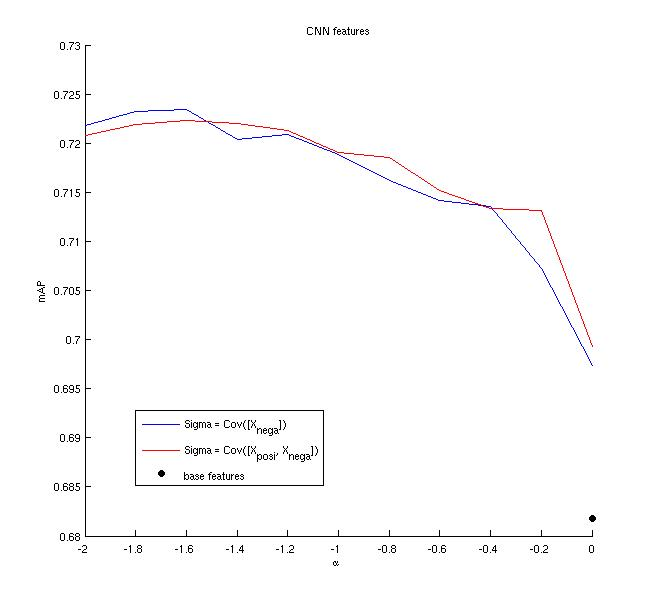
\includegraphics[width=\textwidth]{whitening_cnn.jpg}
\end{subfigure}
\begin{subfigure}[b]{0.45\textwidth}
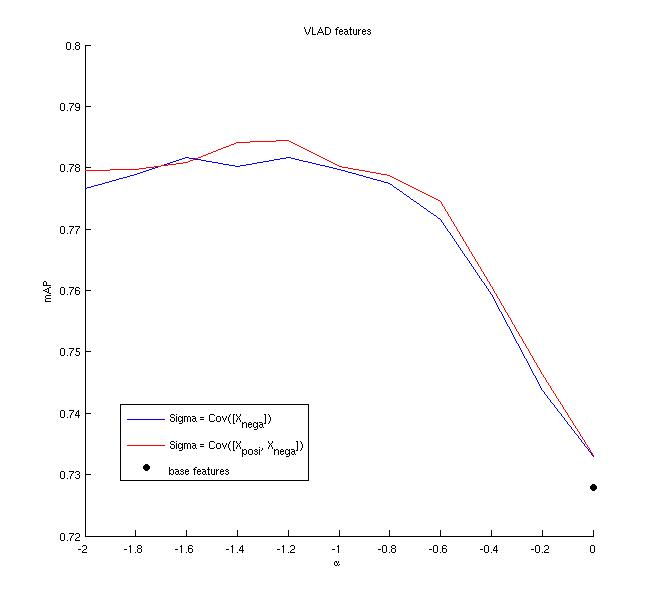
\includegraphics[width=\textwidth]{whitening_vlad.jpg}
\end{subfigure}
\caption{Comparison of mAP for different similarity scores $s_{\alpha}$, varying $\alpha$. On the top, CNN features. At the bottom, VLAD features. On blue, $A$ is the covariance of the negative samples and on red, $A$ is the covariance of the positive and negative samples. In black, the mAP for similarity calculated as inner product of base features.}
\label{salpha:vladcnn}
\end{figure}

\begin{figure}
\centering
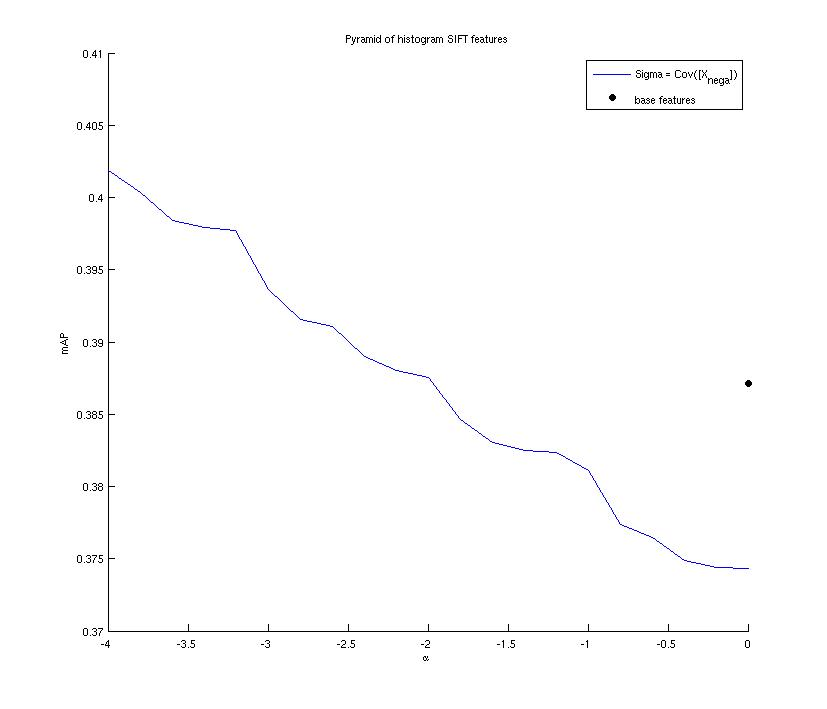
\includegraphics[width=.45\textwidth]{whitening_pyr.jpg}
\caption{Comparison of mAP for different similarity scores $s_{\alpha}$, varying $\alpha$, for spatial pyramid of SIFT descriptors.}
\label{salpha:pyr}
\end{figure}


\bibliographystyle{plain} 
\bibliography{sup}
\end{document}

